% SOURCE: docs/PAPER_DRAFT_INTRO_DIAGNOSIS.md §3 + T4 repairs (Prop 1
% guarantee-iff, cursor streams, state purity; Prop 2 exact c_m) + T5 pins
% (+2.88 definition, probe count) + P13 verdicts + E1/E3 additions.
\section{The Pairing-Divergence Artifact}
\label{sec:f2}

\subsection{Mechanism}

The evaluation question is whether a same-seed comparison preserves the
intended control over training randomness.
Consider two runs launched from the same seed: a method arm $M$ and a
baseline arm $B$. Both draw from process-global RNG streams (PyTorch CPU,
per-device CUDA, NumPy, Python's built-in random). Suppose $M$ executes a probe
at step $t$ that consumes $k$ draws from stream $\sigma$ (a meta-validation
draw, a shuffled evaluation loader, a model re-initialization) and $B$ does
not. If training itself consumes $\sigma$
after $t$, its reads are index-shifted by $k$ on the initially aligned,
equal-consumption prefix, absent further differential consumption, restoration,
or reseeding.
Batch orders or dropout masks can change; the runs remain aligned until an
actual state update differs. Later re-coincidence is not ruled out;
the witnesses document divergence at checked checkpoints or endpoints, not every-update persistence. Single-bit differences are known to drive optimization to
materially different final models \citep{summers2021nondeterminism}; this is a
point-level effect, not a rounding curiosity. Its consequences split by estimand rather than by implementation label.
Without selection, the first failure is loss of the common-random-number
coupling (and hence of the covariance term that can reduce paired variance);
it is not, by itself, a claim of marginal mean bias. Selection on the affected
quantity is different: expected optimism relative to the selected placement's
own mean is nonnegative. The max-minus-placement-average uplift also includes
selection among unequal placement means. In our in-house predecessor a paired RTE
gain of $+2.97$ (4/5 seeds) collapsed to $+0.16$ (2/5) under isolation. That
pair predates the protocol of Section~\ref{sec:repair} and carries no verified
repeat floor (the $+2.97$ arm is by construction the unisolated one), so we
report it at a lower tier than the paper's floor-verified paired results.
Figure~\ref{fig:mechanism} sketches the mechanism.

To keep these claims separate, let $U\sim P$ denote the complete
training-visible random input for one seed and let $Y_M(U)$ and $Y_B(U)$ be
the two endpoint metrics under the intended common input. The marginal method
effect is $\tau=\mathbb E_P[Y_M(U)]-\mathbb E_P[Y_B(U)]$, whereas the paired
estimator uses $Y_M(U)-Y_B(U)$. A displaced arm observes
$\widetilde\Delta=Y_M(TU)-Y_B(U)$ for a stream-shift map $T$, and therefore
\[
\mathbb E[\widetilde\Delta]-\tau
 =\mathbb E_P[Y_M(TU)]-\mathbb E_P[Y_M(U)],\qquad
\operatorname{Var}(\widetilde\Delta)
 =\operatorname{Var}(Y_M(TU))+\operatorname{Var}(Y_B(U))
 -2\operatorname{Cov}(Y_M(TU),Y_B(U)).
\]
Thus a measure-preserving shift ($T_\#P=P$) leaves the marginal mean
unchanged but can reduce the covariance benefit; a finite data-cursor shift
need not be measure-preserving, so Proposition~\ref{prop:pairing} alone does
not assert marginal unbiasedness. For $m$ placements, the pathwise selection
uplift is $H=\max_j\Delta_j-m^{-1}\sum_j\Delta_j\ge0$; calling it a bias
requires the placement average to be the reference estimand. When selection
uses a validation quantity and reporting uses an untouched test quantity, no
one-sided conclusion follows without a transfer assumption.
\subsection{An exact condition}
\label{sec:condition}

The artifact is governed by shared stateful consumption, and the condition
is testable. We state it over \emph{streams} in a deliberately broad sense:
any shared stateful sequence with a monotone cursor, covering PRNG streams and
shared data iterators alike.

\begin{proposition}[Pairing condition]
\label{prop:pairing}
Let $X$ be the complete non-stream training state, including parameters,
buffers, optimizer and scheduler state, modes, caches, and control state;
stream values and cursors are tracked separately. Consider deterministic
executions of the same training program, initially identical in both kinds
of state, with aligned training operations $X_{n+1}=F_n(X_n,z_n)$, where
$z_n$ comprises the stream values read by operation $n$. A \emph{probe}
leaves $X$ unchanged and can affect training only through stream cursors.
Then (i) identical training reads imply bitwise-identical $X$ trajectories;
disjoint probe streams or complete fork--restore suffice. (ii) A probe
advancing one stream by $k\ge1$ shifts its subsequent training reads by $k$
only along an aligned, equal-consumption prefix with no further differential
advance, restoration, or reseeding. The first divergence is the first aligned operation
with common input state $x$ and $F_n(x,z)\ne F_n(x,z')$, not merely different
intermediate values. Later reconvergence is possible. A probe affecting only
streams never subsequently read by training is inert. (iii) Preserving reads
is sufficient, not necessary: distinct read values can induce the same state
update. No necessity or probability-one divergence claim is made.
\end{proposition}

Figure~\ref{fig:hf-boundary} is the paper's cleanest test of
Proposition~\ref{prop:pairing}, because it varies only the probe inside an
unmodified standard framework and reads the result at the bit level. The
matched five-arm audit runs inside the HuggingFace Trainer
\citep{wolf2020transformers} (RoBERTa-base, RTE, 150 steps, deterministic
kernels). Relative to the same reference, an independent repeat, Trainer
periodic evaluation (a sequential sampler and a no-grad forward), and a
CPU random-batch probe remain bitwise identical
(Figure~\ref{fig:hf-boundary}A). Only the CUDA random-batch probe diverges,
because training's dropout later consumes that same stream. A third probe
scheduled after the final update is exactly inert, realizing the boundary case
of Proposition~\ref{prop:pairing}(ii). The reason the evaluation arm survives is
\emph{stream disjointness in this configuration}, not zero consumption: the
eval loader's iterator does draw one 64-bit value from the global CPU stream
at construction (\code{torch/utils/data/dataloader.py:706--710}), the same
draw the BHN witness below turns into a divergence, but training's randomness
here lives on CUDA and on a sampler with its own generator, so no training read
is displaced. The CPU-probe arm measures that directly. A configuration whose
training path did read the global CPU stream, a stochastic collator, or another
RNG-consuming evaluation path need not be clean.

The same experiment answers how large the displacement is.
Across five seeds on each of RTE and MRPC, every CUDA-probe pair diverges and
every independent repeat remains exact (Figure~\ref{fig:hf-boundary}B). The ten
unique task--seed pairs have maximum parameter differences
$5.38$--$6.33\times10^{-4}$ (mean $5.92\times10^{-4}$). Their descriptive
$|\Delta\mathrm{acc}|$ averages $2.58$ points and reaches $5.86$, with
inconsistent sign (4 positive, 6 negative): the artifact does not merely
inflate or deflate, it scatters. At full training length the displacement
persists (Figure~\ref{fig:app-persistence}: mean $1.27$, maximum $2.73$
points), the same order as, and often
larger than, the gaps that method-comparison tables in this literature are
built on.

% Figure 3: empirical HF boundary (single column, 3.3125in).
\begin{figure}[t]
\centering
\IfFileExists{figs/fig3_hf_boundary.pdf}{%
  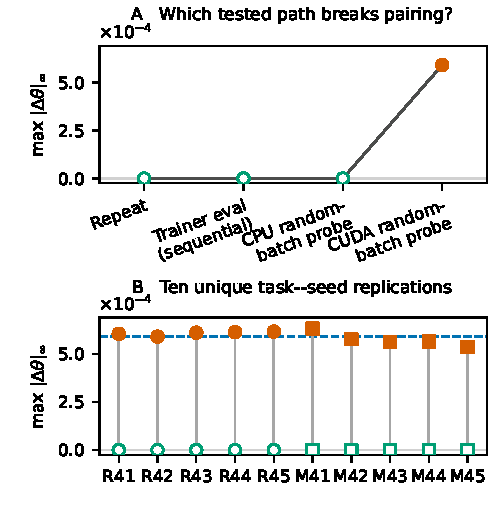
\includegraphics[width=\figwidthcol]{figs/fig3_hf_boundary.pdf}%
}{%
  \fbox{\parbox[c][2.4cm][c]{0.9\columnwidth}{\centering
    Placeholder for \texttt{figs/fig3\_hf\_boundary.pdf}.}}%
}
\caption{\textbf{Among the tested HuggingFace paths, only the probe that touches
training's CUDA random stream breaks exact pairing.} (A) In one matched
five-arm audit, repeat, sequential Trainer evaluation, and a CPU random-batch
probe are exactly zero; the CUDA random-batch probe is nonzero. (B) Across ten
unique task--seed pairs (R = RTE, M = MRPC; digits give the seed), every
repeat is exact and every CUDA probe diverges.
Each value is measured against its corresponding reference; no isolated-HF arm
is implied.}
\label{fig:hf-boundary}
\end{figure}

\subsection{Prevalence, and four byte-level witnesses}
\label{sec:prevalence}

We audited eleven published or field-standard codebases, spanning the
noisy-label and bilevel neighborhood where the diagnosis arose plus
nanoGPT as a reference pretraining loop, in two static-reading waves
(six classic repositories, four official, ${\sim}4{,}400$ stars; five
recent or large-scale). Table~\ref{tab:audit} sketches the verdicts; the
appendix gives file-line citations against pinned commits.

These eleven were \emph{chosen}, not sampled. They are the neighborhood the
diagnosis came from plus a reference pretraining loop, selected because we had
reason to suspect them. Eleven of eleven therefore measures how uniform the
idiom is inside a suspected neighborhood; it is not an estimate of any rate
across deep learning, and no count here is one. The later waves were selected the
same way, for their reach. What the audit does support is narrower: the pattern is
easy to find in code people use, no repository in the core wave isolates any
stream, and the exposure survives into work published through 2024.

The paper's evidence comes at three strengths and Table~\ref{tab:audit} sits in
the middle. \emph{Proven generally}: Proposition~\ref{prop:pairing} holds for
any run meeting its premises. \emph{Shown dynamically}: realized divergence,
confirmed by paired re-execution for four systems only; the tier column marks
which. Those four are not interchangeable either, and we rank them here rather
than let the count stand for them: Meta-Weight-Net and the new nanoGPT
campaign compare repaired arms against a \emph{probe-free} baseline; BHN and DivideMix
verify exact same-configuration floors but contrast two configurations, and
DivideMix's one line moves the mixture's initialization as well as its stream
position; the historical 200-iteration nanoGPT witness had exact floors but
no repaired arm. \emph{Static, and only that}: an EXPOSED verdict says a shared-stream
training consumer and a mid-training consumer of that stream are both present
in the source. It says nothing about whether a published number is wrong, and
nothing about any particular comparison, because desynchronizing a pair
additionally needs that consumer to fire \emph{differently} between the arms.
Where it fires identically in both, the shared stream is a path this comparison
does not walk. Arm-differential firing is what the four re-executed witnesses
show and a static reading cannot. The harvest measurements of
Section~\ref{sec:harvest} distinguish historical single-codebase calibration
from a separate nanoGPT calibration/held-out check.

\begin{table}[t]
\centering
\scriptsize
\setlength{\tabcolsep}{2.2pt}
\begin{tabular}{@{}p{0.33\columnwidth}p{0.49\columnwidth}p{0.12\columnwidth}@{}}
\toprule
Codebase & Exposure mechanism & Tier \\
\midrule
L2RW official (ICML'18) & eval consumes train iterator & static \\
L2RW PyTorch reimpl. & per-step re-init; shuffled eval & static \\
MW-Net official (NeurIPS'19) & per-step re-init + meta loader & \textbf{dyn.} \\
DivideMix official (ICLR'20) & unseeded GMM $\leftrightarrow$ mixup & \textbf{dyn.} \\
Co-teaching official (NeurIPS'18) & eval-active dropout (CUDA) & static \\
MAML reimpl. \citep{finn2017maml} & mid-epoch shuffled test loader & static \\
RENT official (ICLR'24) & on-device multinomial (CUDA) & static \\
BHN official (ICML'23) & per-epoch loader rebuild + probe & \textbf{dyn.} \\
TopoFilter official (NeurIPS'20) & per-epoch probe over shuffled loader & static \\
CRUST official (NeurIPS'20) & train-mode gradient probe & static \\
nanoGPT (60.7k$\star$) & eval shares training's randint & \textbf{dyn.} \\
\bottomrule
\end{tabular}
\caption{Eleven audited codebases, eleven exposures; none isolates any
stream (negative grep, independently re-verified); ``dyn.'' = divergence
confirmed by re-execution.}
\label{tab:audit}
\end{table}
All eleven are exposed; none
constructs a dedicated generator object to isolate any stream (verified by
negative grep), and seeding, where attempted, is a single global call
(one reimplementation never seeds torch; CRUST \citep{mirzasoleiman2020crust} defaults to none). Every
verdict was re-derived by an independent second reading against
pinned commits (SHAs in the appendix): none refuted, two strengthened, since
TopoFilter's \citep{wu2020topofilter} probe consumes a full shuffled-loader permutation per
epoch, and stock DivideMix never seeds NumPy, so exact same-seed reruns
of the released code are irreproducible past warm-up. Four of the
eleven (Meta-Weight-Net, nanoGPT \citep{karpathy2022nanogpt},
DivideMix, and BHN) are
additionally confirmed by dynamic paired re-execution (the L2RW
reimplementation was re-executed only for signal-scale measurements, not a
paired-divergence test), and in all four, paired runs diverge exactly when the
static analysis predicts. Divergence and repair are separate results, verified
on different sets, and we state the split rather than average over it.
For Meta-Weight-Net, a repaired arm run against a \emph{probe-free}
baseline was found SHA-256 identical to it (5/5 seeds). For
BHN and DivideMix we re-executed a repaired arm and verified its
same-configuration floor exactly, but the reported contrast is between two
configurations rather than against a probe-free run. The historical nanoGPT
witness had no repaired arm; the new campaign below adds that comparison.
The DivideMix witness localizes the cause to one
line: four arms of the official code (CIFAR-10, 50\% symmetric noise, 12
epochs) under one byte-identical harness that seeds NumPy and pins kernels,
neither of which the release does, differ only in whether the co-divide GMM
draws its initialization from the shared global NumPy stream or from a pinned
sklearn random state. Both repeat floors are exact; all four logs are
byte-identical through the ten warm-up epochs, where the differing line
never executes, then separate at the first co-divide epoch, ending
$0.73$ points apart on the printed final accuracy. This localizes the cause to
that line and no further: pinning the mixture's random state changes its own
initialization as well as where its draws come from, so the two arms differ
both in the split the mixture produces and in the stream position training
inherits. DivideMix is therefore a witness that the line matters, not a clean
separation of cursor displacement from re-initialization; the state-pure probes
of Proposition~\ref{prop:pairing} are the other three. The BHN witness isolates a
still smaller consumption: the single 64-bit
seed its mid-training test loader draws when its iterator is constructed
(the loader is unshuffled and eval-mode; that seed is its \emph{only}
shared-stream draw). One native generator argument to that loader removes
exactly that draw, method semantics untouched. In four arms (official
ResNet-34, CIFAR-10, 12 epochs; both repeat floors weight-exact),
per-epoch weight hashes are identical through epoch 1 and diverge exactly
at epoch 2, the first epoch whose shuffle order the probe's stream
position can reach, ending $1.93$ points apart on the printed test
accuracy: a single 64-bit draw, in official ICML-2023 code. The same
witness holds at the \emph{full shipped $200$-epoch protocol}: the
isolated pair stays bitwise-identical through all $200$ epochs, and the
configurations end at $82.68$ vs.\ $83.03$. The gap narrows to $0.35$
points but the mechanism is intact at convergence. The fourth witness
leaves supervised vision entirely: four nanoGPT arms at $200$ iterations
(\code{shakespeare\_char}, fp32) differ only in whether the loss-estimation
pass draws its batches from the same \code{randint} stream training uses,
both same-configuration repeat floors are exactly zero, and the
evaluation-versus-no-evaluation contrast reaches
$\max|\Delta W| = 3.3\times10^{-2}$ (floors in Table~\ref{tab:floors}).

Three structural observations follow. First, within this neighborhood the
pattern is structural, not incidental: the bilevel implementations draw meta-batches from a
shuffled loader on the global generator and rebuild the network
every step, so the probe fires \emph{every training step}; the artifact is a
property of the method as implemented, not of an evaluation harness. Second,
the mechanisms are diverse enough to defeat spot-checking: a data-pointer
variant needing no RNG at all (official L2RW's evaluation consumes batches from
\emph{training's own iterator}, and its pipeline re-seeds from entropy, so its
same-seed-list comparisons were never seed-controlled), an eval-active-dropout
variant (Co-teaching), and a variant whose shared draws are on the CUDA
stream (RENT). Third, the pattern
persists unchanged into ICML 2023, ICLR 2024, and the 60.7k-star reference
pretraining loop.

The reach extends past the noisy-label neighborhood, and divides along the
isolation boundary of Section~\ref{sec:repair}. A second wave reads twelve
field-standard training loops at file--line resolution
(Table~\ref{tab:fieldwide}). Ten are exposed: the reference vision recipe (timm
\citep{wightman2019timm}, whose periodic validation desynchronizes the next
epoch's shuffle, reproduced under torch~2.11), a widely copied diffusion
template \citep{lucidrains2020ddpm}, single-file RL, LLM finetuning, five
recent selection methods (Sel-CL, MLC, ProMix, UNICON, DISC), and InfoBatch:
its NumPy pruning reseed does not protect main-process torch augmentation
from the unshuffled evaluation loader's base-seed draw. Two guard the audited
RNG channel (a fixed-noise DCGAN buffer and deterministic Stable-Baselines3
evaluation with a separate, privately seeded environment); this does not
certify state purity, since DCGAN visualization updates BatchNorm buffers. A third wave
probes five flagship 2023--2026 stacks, where the boundary is a design choice
rather than an era: SDXL's in-loop logging is exposed by default; in TRL and a
diffusers script a single flag decides between exposed and guarded; OLMo-core
and MMSelfSup guard the audited RNG paths under their stated configuration conditions.
Neither wave enters the eleven-of-eleven count.

\subsection{The printed gap moves, and selection harvests it}
\label{sec:harvest}

Prevalence shows preconditions; a moved gap and a harvested one show
consequence. The
claim is tiered like the evidence: the static audit establishes the
\emph{precondition}, the byte-level witnesses the \emph{desynchronization},
the harvest the \emph{uplift in the selected reported quantity}. We claim
no audited paper's published result is wrong, only that the instrument
can be silently defeated, and that selection on the reported quantity can
produce a one-sided reported uplift. In Meta-Weight-Net's official codebase, with model,
meta-network, and RNG topology untouched and the repeat floor weight-exact
(model and meta-network SHA-identical across same-seed reruns, five seeds),
we insert one semantically inert random-permutation draw during
training and recompute the method-versus-baseline gap the paper's tables
would print. The gap moves by 1.78 points on seed 1 and 1.16 points on seed
2, in opposite directions. We make no claim about MW-Net's true ordering
against its baseline (our protocol is shortened); the claim is that in a
NeurIPS-published method's official code, a single RNG draw moves the
printed comparison by more than a point above an exact floor.

% Figure 2: harvest scatter + extreme-value growth. Rendered two-up at the
% full 6.5in measure, so it is placed at its native width and not scaled.
% Falls back to the shared column width anywhere that does not define this.
\providecommand{\figwidthharvest}{\figwidthcol}
\begin{figure}[t]
\centering
\IfFileExists{figs/fig2_harvest.pdf}{%
  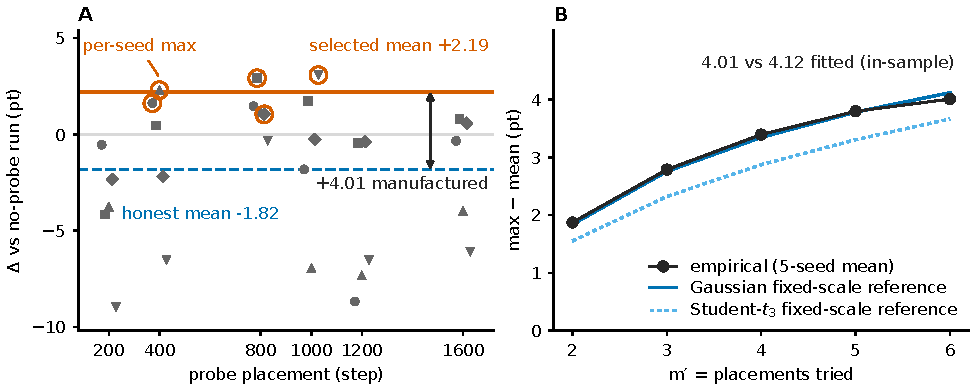
\includegraphics[width=\figwidthharvest]{figs/fig2_harvest.pdf}%
}{%
  \fbox{\parbox[c][2.97cm][c]{0.9\columnwidth}{\centering
    Placeholder for \texttt{figs/fig2\_harvest.pdf}.}}%
}
\caption{\textbf{Selection turns bidirectional divergence into a one-sided report.}
Across five seeds and six probe placements, the honest mean is $-1.82$ points,
whereas selecting each seed's best placement reports $+2.19$, manufacturing
$+4.01$. The growth over the number of tried placements tracks the finite-$m$ Gaussian benchmark in this grid rather than its asymptotic form
(Proposition~\ref{prop:harvest}). This historical grid comes from one codebase
on one dataset, with $c_m\sigma$ serving as a conditional, same-sample
benchmark whose predictive scope is assessed separately.}
\label{fig:harvest}
\end{figure}

To quantify the reporting consequence of placement selection, we use an
idealized scaling benchmark: under the iid-Gaussian null, selection over
placements has expected uplift $c_m\sigma$. Its empirical calibration is
setting-specific. The historical measurements use one codebase
(Meta-Weight-Net's official release) and dataset (CIFAR-10). The separate
nanoGPT check below estimates its own scale from calibration seeds before
held-out evaluation, assessing within-setting prediction rather than
transfer across architectures, datasets, or tasks.
Across 5 seeds $\times$ 6 placements on the same machine
(shortened protocol: Meta-Weight-Net official code on a $10{,}000$-image
CIFAR-10 subset at $40\%$ symmetric noise, $20$ epochs of $100$ steps, giving
mean within-seed sample SD $\bar\sigma = 3.25$ points, computed across
placements with denominator $m-1$ (\code{ddof=1}); Figure~\ref{fig:harvest}),
the probe \emph{hurts} on
average (honest mean $-1.82$) yet per-seed best-placement selection
reports $+2.19$, an observed $+4.01$ uplift over the placement average.
The decomposition below separates reporting optimism from systematic
placement effects; these five seeds do not identify their population shares.

\begin{proposition}[Harvest size]
\label{prop:harvest}
For integrable paired gaps $D=(D_1,\ldots,D_m)$, set $\mu_j=\mathbb E D_j$
and let $J$ be a fixed tie-broken maximizer of $D_j$. With arbitrary means
and dependence, selected-placement optimism satisfies
\[
\mathcal O:=\mathbb E[D_J-\mu_J]
\ \ge\ \max_j\mu_j-\mathbb E\mu_J\ \ge\ 0.
\]
The reported uplift $H(D)=\max_jD_j-m^{-1}\sum_jD_j$ instead obeys
$\mathbb EH(D)=\mathbb E[\mu_J-\bar\mu]+\mathcal O$; the first term need
not be positive. Common additive components cancel from $H$.
In the equal-mean Gaussian special case $D_j=a+C+\sigma Z_j$, with $\sigma\ge0$,
integrable common $C$ and i.i.d.\ standard normals $Z_j$,
$\mathbb EH=\mathcal O=c_m\sigma$, where $c_m=\mathbb E\max_j Z_j$
($c_6=1.27$). These are classical selection and order-statistic identities,
not a new universal Gaussian law.
\end{proposition}

\evidencefloats{}
The descriptive comparison is $\RevHarvest$ points of observed uplift
against $c_6\bar\sigma=\RevPrediction$, using the same placement outcomes
to estimate $\bar\sigma$, the mean within-seed sample SD. Under the
equal-mean iid-normal model, dividing each SD by its normal expectation
factor $c_4(m)$ gives $\RevCorrectedPrediction$. Exact quadrature yields
uncorrected ratios $0.9734$, $1.1463$, $1.0075$ across the shortened,
realistic-evaluation and full-best campaigns; the corrected ratios are
$0.9262$, $1.0775$, $0.9282$. Figure~\ref{fig:ratios} jointly recomputes
numerator and denominator over every ordered whole-seed bootstrap sample.
The corrected full-best interval is $[0.8665,0.9776]$: it excludes one, but
27 resamples of three seeds are a discrete sensitivity analysis, not reliable
model rejection or calibrated population coverage.

The placement effect reported at $p=0.049$ in Appendix~C relies on exchanging
fixed training positions and is conditional on that exchangeability null.
Treating observed column means as fixed offsets changed a legacy simulation
ratio from $1.00$ to $1.04$; this is a fitted-offset sensitivity, not proof
that the iid formula tolerates offsets. Appendix~C now gives a distribution-free
offset bound and a variance decomposition showing exactly how offsets and
contrast covariance enter the fitted scale.

We additionally simulate the complete fit-and-select procedure, re-estimating
all SDs in each of 100,000 Gaussian and variance-matched $t_3$ datasets.
For the $5\times6$ design, the corrected-ratio reference intervals are
$[0.8087,1.1979]$ and $[0.7251,1.3014]$, respectively. Their overlap shows
why comparing expected-maximum constants with a fixed fitted SD cannot
establish the residual distribution. The earlier growth curve is retained as
a same-grid descriptive comparison, not distributional or predictive validation.
The
harvest is consistent with an extreme-value benchmark for divergence noise,
but Proposition~\ref{prop:pairing}(ii) alone implies neither a fresh-seed law
nor Gaussian or independent placement residuals. Three limits bound how far
the agreement may be read. $c_m\sigma$
prices what a \emph{reporting practice} harvests on average over seeds rather
than what any one run will show. $\sigma$ is heteroscedastic across seeds
($1.4$--$4.6$) and does not transport between them, so a preregistered
leave-one-seed-out test misses a held-out seed's harvest by $2.17$ points on
average\evidencefigs{}. And Proposition~\ref{prop:harvest} prices selection
performed \emph{on the affected quantity}: where a validation quantity selects
and an untouched test quantity is reported, the direction and magnitude of transfer remain unestablished
by the present evidence. The preregistered bridge gives a selected
test delta of $+\RevEOneMean$. Its original preregistered seed-level $t$
interval is $[\RevEOneTLow,\RevEOneTHigh]$; the separate reviewer-requested
100,000-draw seed-cluster bootstrap gives
$[\RevEOneBLow,\RevEOneBHigh]$, also including zero. The within-seed
centered correlation is $\RevEOneR$ (Table~\ref{tab:e1}); centering removes
all seed means and does not identify the baseline's causal contribution.
We therefore
claim a guaranteed nonnegative expected optimism only for selection on the
reported quantity itself. Positive validation--test Pearson correlation
alone does not guarantee positive test-selection optimism (Appendix~C).

The mechanism also appears with an unmodified shuffled monitoring loader
(MW-Net, $45{,}000$ training images, $12$ epochs): its two seed draws
produce $+0.45$ points of max-minus-mean uplift across five seeds and five
placements. The two directly checked isolated model/meta-network pairs
match the never-probed baseline. At the full $120$-epoch protocol,
all twelve shared placement--seed pairs diverge; best-of-four uplift is
$+0.16$ points, and the three checked repaired pairs match baseline.
These are scoped endpoint comparisons, not all-placement trajectory
verification; best and final are endpoints of the same three-seed campaign.
Appendix~\ref{sec:extended-harvest} preserves the protocols, effect sizes
and verification details; Figure~\ref{fig:ledger} records the coverage.

\paragraph{Independent-setting, frozen nanoGPT prediction check.}
A separate 2,000-update campaign uses five prespecified probe placements
($200,500,900,1300,1700$), 16 calibration seeds and 16 disjoint held-out seeds.
For each seed, $D_j=L_{\rm baseline}-L_{{\rm shared},j}$ uses the same fixed
validation panel, and $H=\max_jD_j-\bar D$. Calibration alone fixes
$c_5\overline{s}/c_4(5)=0.00388406$ loss units before held-out runs;
the observed held-out mean is $0.00343060$. Independently bootstrapping
whole seed vectors in each split (20,000 draws) gives approximate 95\%
intervals $[0.00327501,0.00449714]$ for the prediction and
$[0.00279334,0.00407564]$ for the observed mean. Observed minus predicted
is $-0.00045346$ ($-11.67\%$), with interval
$[-0.00134285,0.00043370]$. Inclusion of zero establishes neither equivalence
nor the conditional Gaussian model. This is a new setting's held-out
mean-prediction check, not validation-to-test transfer or a per-run forecast.
All 160 seed--placement shared paths diverge and all 160 isolated paths
match their probe-free baseline at the checked state resolution; two
repeats per path are verification, not additional independent observations.
Appendix~\ref{sec:nanogpt-supplement} reports the prespecified uncorrected
sensitivity and exploratory selected-score, placement and influence checks.

\subsection{Kernel nondeterminism, and the repair protocol}
\label{sec:repair}

Closing every shared-stream leak is still not sufficient for pairing. With
identical training mathematics and no RNG sharing, nondeterministic GPU
kernels alone bifurcate same-seed cross-arm trajectories, a documented
layer \citep{zhuang2021randomness} for which we claim no novelty, and one
that repeat checks help distinguish from deterministic stream displacement:
a nonzero same-configuration floor detects nonrepeatability, whereas a
deterministic stream shift can leave repeats exact while moving a cross-arm
pair. A finite zero floor does not rule out all nondeterminism. The layer
is material: in an under-tuned CIFAR-100 regime
(constant lr, no augmentation, TF32), same-seed raw candidates across arms
differed by up to 11.7 points; in our NLP suite, trajectories that were
bitwise-identical for the first half epoch subsequently bifurcated by 13.7
points on CoLA. Seeds alone therefore never
establish exact pairing; repeat checks must accompany the isolation and
state-purity premises.
The repair has three requirements with different costs, and they are
checkable in the order given. Probe isolation is often a small code change;
deterministic kernels, per-path reruns, state capture, and storage can carry
substantial runtime or platform costs.

\begin{enumerate}\itemsep1pt\parskip0pt\topsep2pt
\item \emph{Isolate every probe.} Each mid-training consumer of randomness runs
inside PyTorch's fork-rng context manager \citep{pytorch_forkrng} or uses
dedicated generator objects, leaving \emph{all} training streams untouched.
All of them means all: fork-rng covers only torch's CPU/CUDA generators, so
NumPy, Python's built-in random, and library-internal draws need dedicated or
pinned states (DivideMix's repair pins sklearn's); a shared \emph{data cursor}
needs its own iterator (official L2RW consumes no RNG at all); and the probe
must write no training-visible state, state purity in the sense of
Proposition~\ref{prop:pairing}. Figures~\ref{fig:hf-boundary}
and~\ref{fig:app-realeval} show the boundary this draws.
\item \emph{Pin kernels.} Deterministic kernels for any run used in a paired
claim; nondeterministic ones break pairing with no RNG sharing at all.
\item \emph{Verify a zero repeat floor on every materially distinct path.}
Rerun each arm and configuration whose kernel, control flow, precision,
stochastic consumer, or probe differs, under the identical seed and
configuration. Require the difference to be exactly zero at the resolution of
the intended claim before interpreting a cross-arm delta (per-campaign floors:
Table~\ref{tab:floors}). A metric floor supports only a metric claim; weight
or full-state claims require the corresponding hashes. The floor turns ``we
set seeds'' into a measurement on the tested path, not a universal proof of
determinism.
\end{enumerate}

\noindent In released code the first requirement is often a small wrapper, and the
three systems where we re-executed a repaired arm show the shape of it.
Meta-Weight-Net's per-step probe needs the probe body wrapped in
\code{with torch.random.fork\_rng(devices=[device]):} (\code{devices=[]} on
CPU), after which the isolated arm
is SHA-256 identical to the never-probed baseline on 5/5 seeds. BHN's
mid-training test loader draws one 64-bit seed at iterator construction, removed
by passing \code{generator=torch.Generator().manual\_seed(0)} to that
\code{DataLoader}, method semantics untouched. DivideMix's co-divide GMM draws
from global NumPy, pinned by \code{GaussianMixture(..., random\_state=0)}. Each
exposure in the field-wide wave maps to one of those three shapes, a
\code{fork\_rng} wrapper for an in-loop evaluation or sampling call, a
dedicated \code{generator=} for a probe's loader, or a pinned state for a
library that reads a global stream. Apart from the new nanoGPT campaign
above, we have not re-executed repaired arms in that wave; for those
remaining entries the mapping is a prescription, not a result.

\noindent Table~\ref{tab:floors} records the actual repeat evidence and its
resolution, including absent floors. Historical NLP zero cells and the
pre-protocol in-house comparison are excluded from certificate counts.
A floor from one tested path is not silently transferred to a distinct arm.
The isolation clause is verified on the witness codebase itself:
fork-rng isolation returns model and meta-network to SHA-256 identity with
the never-probed baseline, on five seeds at the shortened protocol and three
at the full (probes verified to fire).

\subsection{The repair's certificate: a certified no-op}
\label{sec:receipt}

The repair gives a conditional no-op result, illustrated by a guarded
weight-averaging endpoint that may serve its raw candidate. Candidate
maintenance and evaluation must satisfy Proposition~\ref{prop:pairing};
repeat floors test the implementation but do not replace its premises.

\begin{corollary}[Certified no-op]
\label{cor:noop}
Under the deterministic pairing protocol, state-pure and stream-isolated
candidate maintenance gives champion $=$ raw $\Rightarrow$ served parameters
and buffers are bitwise identical to the paired baseline endpoint, so every
deterministic reported metric delta is exactly zero. The reverse implication
requires the additional checked premise that every non-raw candidate differs
from raw in at least one parameter bit; EMA or frozen candidates may collide
exactly and this premise is not inferred merely from training having moved.
\end{corollary}

The certificate requires the full conjunction of premises, not merely a
logged raw champion and a zero metric. Historical tuned-regime observations
are retained in Table~\ref{tab:certreg} as descriptive results, with missing
floors excluded from certificate counts. Direct weight comparisons, metric
equality and full-state verification remain distinct evidence categories
(Figure~\ref{fig:ledger}). Detailed averaging, monitor and meta-signal analyses
are in the appendix; the main contribution is the pairing diagnosis and
the operational checks that make its repair testable.
